\documentclass[11pt]{article}
\usepackage{fancyhdr}
\usepackage[usenames, dvipsnames]{xcolor}
\usepackage{graphicx,hyperref}
\hypersetup{
	colorlinks,
	citecolor=black,
	filecolor=black,
	linkcolor=black,
	urlcolor=black
}
\newcommand{\HRule}{\rule{\linewidth}{0.5mm}}
\pagestyle{fancy}
\lfoot{\small \color{gray}Tom Peerdeman - 10266186}
\cfoot{\thepage}
\rfoot{\small \color{gray}Ren\'e Aparicio Sa\'ez - 10214054}
\lhead{\small \color{gray}Opgave 4: Beschadigingen in een FAT-12}
\begin{document}
	\begin{titlepage}
	\begin{center}
		\textsc{\Large Besturingssystemen}\\[0.5cm]
		\HRule \\[0,4cm]
		\textsc{\huge \bfseries FAT-12 errors}
		\HRule \\[8cm]
		\begin{minipage}{0.4\textwidth}
			\begin{flushleft}\large
				\emph{Auteurs: Tom Peerdeman \& Ren\'e Aparicio Saez}\\
			\end{flushleft}
		\end{minipage}
		\begin{minipage}{0.4\textwidth}
			\begin{flushright}\large
			\emph{Datum: 25-05-2012\\\'}\\
			\end{flushright}
		\end{minipage}
	\end{center}
	\end{titlepage}

	\tableofcontents
	\newpage

	\section{Inleiding}\label{sec:inleiding}
	Een FAT (File Allocation Table) is een single linked list. Deze bevat 'entries' voor clusters. Iedere entry geeft aan waar de volgende cluster gevonden kan worden. Of, als er geen nieuwe clusters meer zijn, dat alle clusters opgehaald zijn. Deze clusters samen vormen een file. Dit is een eenvoudige en betrouwbare manier om files op te slaan. Echter kunnen er wel fouten optreden in de FAT. Specifiek wordt er gekeken naar de 12 bits variant, FAT-12.
	\begin{figure}[h]
		\begin{center}
		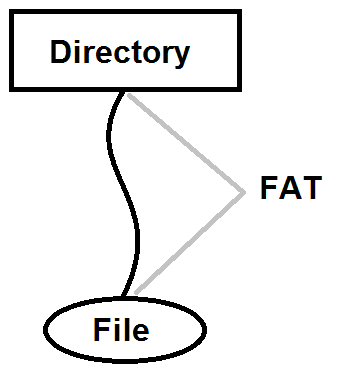
\includegraphics[width=0.4\textwidth]{fatgoed.png}
		\caption{Schematische weergave van de werking van een 	FAT}
		\end{center}
	\end{figure}

	\newpage

	\section{Fouten in de FAT}\label{sec:fout}
	\subsection{Fouten overzicht}\label{sec:overzicht}
	Er zijn verschillende soorten fouten die kunnen optreden in een FAT-12. Sommige fouten zijn eenvoudig op te lossen en op te sporen.\\\\
	Enkele fouten in de FAT die zijn op te sporen zijn bijvoorbeeld:
	\begin{itemize}
		\item Dubbel gebruik van een deel van de FAT
		\item Een file die twee keer voor komt in \'e\'en directory
		\item Een file die twee keer voor komt in verschillende directories
		\item Geen overeenkomende lengte in de directory en het aantal clusters
		\item Loops in de FAT
		\item Incorrect eindigende link
		\item Een file komt nog voor in de FAT maar staat niet meer in de directory
	\end{itemize}
	Daarnaast zijn de volgende fouten niet op te sporen:
	\begin{itemize}
		\item Een file die bestaat in de directory maar niet in de FAT
	\end{itemize}

	\newpage

	\section{Ge\"implementeerde fouten}\label{sec:impfout}
	\subsection{Dubbel gebruik van een deel van de FAT / Dubbele file}\label{sec:dubbel}
	Een deel van de FAT mag niet dubbel gebruikt worden. Als dit wel gebeurd en \'e\'en van de twee (of meerdere) files wordt verwijderd dan wordt ook automatisch de bijbehorende FAT geleegd. De nog wel bestaande identieke file(s) zullen dan niet meer werken. Hiertoe wordt bijgehouden welke clusters al gelezen zijn. Wordt een cluster dubbel gelezen dan bestaat een file twee of meerdere malen. Of twee verschillende files gebruiken hetzelfde deel van een FAT. Bestaat een file twee keer, dan hebben ze dezelfde lengte en exact dezelfde FAT-index. Dit zou opgelost kunnen worden door de files samen te voegen tot \'e\'en. Is de lengte niet hetzelfde en verschillen er fat-indices dan wordt slechts een deel van de fat dubbel gebruikt. Dit kan opgelost worden door bijvoorbeeld de tweede file niet weg te schrijven, echter zal deze file dan dus verloren raken. 

	\subsection{Geen overeenkomende lengte}\label{sec:lengte}
	De lengte van de file is bekend, echter kan het voorkomen dat deze lengte niet overeenkomt met de FAT. Er treedt dan een fout op. De lengte in de FAT kan ofwel te lang ofwel te kort zijn. Is de lengte te lang dan is het aantal gelezen clusters groter dan het aantal clusters dat de file zou horen te hebben. Is de lengte te kort dan zijn er te weinig clusters gelezen dan zou moeten, de FAT denkt aan het einde te zijn terwijl dit niet zo is. Als de lengte te lang is kan het probleem allicht opgelost worden door te proberen de file te schrijven als het juiste aantal in de FAT is bereikt. De clusters die nog zouden volgen volgens de FAT worden geleegd. Echter kan de file dan alsnog kapot zijn. Als de lengte te kort is dan valt er niks te doen en is het beter om de clusters te legen en de (kapotte) file te verwijderen.

	\subsection{Loops}\label{sec:loops}
	In een FAT kunnen loops optreden. Er wordt dan een deel van de FAT meerdere malen aangeroepen. In een FAT mag dit niet voorkomen (zie \ref{sec:dubbel}). Om een loop op te sporen moet worden gekeken of een cluster dubbel gelezen wordt door \'e\'en file. Dit gebeurt in dezelfde methode waarin al wordt gecheckt of een file dubbel voor komt. Wordt er een loop waargenomen dan moet deze worden verbroken, anders wordt er eeuwig doorgeloopt en wordt dezelfde foutmelding ook eeuwig gegeven. De FAT zou alleen hersteld kunnen worden als de cluster vlak voor de herhaling van een cluster die al geweest is de laatste cluster zou zijn. Deze cluster moet dan voortaan verwijzen naar een terminerende cluster. Als deze cluster niet de laatste cluster van de file is kan er niet met zekerheid bepaald worden welke cluster er zou moeten volgen.

	\subsection{Incorrecte eindigende links}\label{sec:links}
	Sommige links uit de FAT kunnen het einde incorrect aangeven. De aangegeven link zou bijvoorbeeld nog verder willen gaan, terwijl er geen nieuwe clusters meer worden verwacht. Dit is te herstellen door de cluster die als laatst verwacht wordt aan te geven als laatste cluster.

	\newpage

	\section{Overige fouten}\label{sec:overige}
	\subsection{Een file die niet voor komt in de FAT}\label{sec:dir}
	Het kan voorkomen dat een file niet (meer) bestaat in de FAT. Dit kan bijvoorbeeld gebeuren als \'e\'en van twee exact dezelfde files wordt verwijderd (zie \ref{sec:dubbel}). Het is niet mogelijk om dit te herstellen, de file kan immers niet meer opgebouwd worden via de clusters uit de FAT.

	\subsection{Een file die nog wel in de FAT staat maar niet in de directory}\label{sec:fat}
	Het is mogelijk dat een deel van de FAT nog in gebruik is maar de file waar ze bij horen niet meer bestaat. Het is niet eenvoudig om dit te herstellen omdat het aantal clusters waar het om gaat niet bekend is, aangezien er geen file meer is.

	\subsection{Vrije ruimte staat niet gemarkeerd als vrije ruimte in de FAT}\label{sec:vrij}
	Alle ruimte die niet gebruikt wordt door de FAT om files mee te maken is bezet. De vrije ruimte zou gebruikt kunnen worden om nieuwe files in op te slaan. Maar het is mogelijk dat deze vrije ruimte als bezet wordt aangegeven. Dit is alleen op te lossen als zich geen fouten voordoen in de FAT. Anders kan je zonder mogelijkheid weten of de ruimte vrij zou horen te zijn of gebruikt zou moeten worden door een file die behoord bij een kapot deel van de FAT.

	\subsection{0x05 / 0xE5}\label{sec:0xE5}
	Tijdens de experimenten bleek een deel van de FAT altijd gebruikt te worden maar niet bij een specifieke file te horen. Het bleek te gaan om clusters met de naam 0x05 of 0xE5. Een cluster krijgt deze naam toegewezen als de bijbehorende file verwijderd is. Op deze manier is het eventueel mogelijk om de file te recoveren. In het programma worden clusters die 0x05 of 0xE5 heten genegeerd. 

	\newpage

	\section{Makefile / setup}\label{sec:setup}
	Om het programma te laten werken moeten alle files uit de gecomprimeerde map woorden gehaald en in een directory worden geplaatst. Vervolgens dient er via een commandshell genavigeerd te worden naar deze directory. Als de gebruiker in de juiste directory zit moet in de shell het commando 'make setup' worden uitgevoerd. 
Hiermee worden de juiste mappen aangemaakt die nodig zijn om de output in op te slaan. Als het eerste commando is uitgevoerd kan het volgende commando worden ingetypt. Dit is het commando 'make'. Alle code wordt nu gelinkt en gecompileerd tot twee werkende programma's: fat-checker \& fat-extracter. Zodra dit is gebeurd kunnen de programma's gebruikt worden. De meest eenvoudige manier om alle dick-images in \'e\'en keer uit te voeren en alle uitvoer weg te laten schrijven is door het commando 'make run' te gebruiken. Hierbij worden eerst alle files uit de disk-images weggeschreven door het programma fat-extract. De files worden per disk-image in de directory 'extract' opgeslagen. In de directory 'out' staan twee directories, de uitvoer voor het wegschrijven van de files staat in de directory 'extracter'.
Vervolgens wordt het tweede programma, fat-checker, uitgevoerd. De uitvoer van dit programma wordt weggeschreven in de directory 'checker', de tweede directory in 'out'.
	
	\newpage

	\section{Resultaten}\label{sec:result}
	
	\subsection{Disk-image3}\label{sec:disk3}
	Disk-image3 is de enige disk-image waar geen fouten bij optreden. Alle files worden goed weggeschreven. De files zijn respectievelijk 'README.TXT' en een directory 'FILES'. In deze directory bevinden zich twee andere directories: 'LOGOS' en 'POSTERS'. In de directory 'POSTERS' staan twee files, respectievelijk 'SANTOSO.PDF' en 'SPINNATO.PDF'. In de directory 'LOGOS' bevinden zich drie directories: 'CSP', 'ICCS' en 'UVA'. De directory 'CSP' bevat twee files: 'CSP.PNG' en 'SCS-BLUE.gif'. De directory 'ICCS' bevat vier files: 'ICCS2010.GIF', 'SHIRT.PNG', 'SHIRT-BL.PNG' en 'STICK.GIF'. Tenslotte bevat de directory UVA vier files: 'ACRONIEM.GIF', 'ACRONIEM.PNG', 'CENTRAAL.GIF' en 'UVA300.PNG'.

	\subsection{Disk-image1}\label{sec:disk1}
	Bij de eerste disk-image zijn FAT1 en FAT2 niet gelijk bij index 74. Hij bevat twee verwijderde entries met de namen: 'åEWFOL~1' en 'åILES'. Dit resulteert erin dat de directory die eigenlijk 'FILES' hoort te heten niet wordt weggeschreven. De directories en files die hierin staan worden hierdoor dus ook niet weggeschreven en gezien als 'loose file/directory'.

	\subsection{Disk-image2}\label{sec:disk2}
	De tweede disk-image bevat inconsistenties in de FAT op index 62 en indices 219 t/m 225. Bij het controleren van de files blijkt dat index 62 verwijst door naar een volgende cluster terwijl verwacht werd dat dit de laatste cluster zou zijn. Er is dus een fout met de lengte in de FAT en het resulteert in het niet kunnen schrijven van de file 'SHIRT.PNG'. Index 219 verwijst naar een lege cluster. Dit resulteert in het niet kunnen wegschrijven van de file 'STICK.GIF'.

	\subsection{Disk-image4}\label{sec:disk4}
	De vierde disk-image bevat geen inconsistenties in de FAT. Bij het controleren van de files blijken hier wel fouten op te treden. De file 'ICCS2010.GIF' kan niet worden weggeschreven omdat de lengte van deze file te lang is. Er zijn meer clusters dan wordt verwacht. De file 'SHIRT-BL.PNG' bestaat dubbel, maar wordt wel weggeschreven. Er bevinden zich ook twee ongebruikte files in de FAT die niet worden weggeschreven, dit zijn 'SCS-BLUE.gif' en 'STICK.GIF'. 

	\subsection{Disk-image5}\label{sec:disk5}
	De vijfde disk-image bevat \'e\'en inconsistentie in de FAT op index 1523. Bij het controleren van de files blijkt dat de lengte niet te kloppen. Er wordt verwacht dat het einde van de clusters is bereikt maar er wordt nog doorverwezen naar een volgende cluster. Dit resulteert in het niet kunnen wegschrijven van de file 'SANTOSO.PDF'.

	\subsection{Disk-image6}\label{sec:disk6}
	De zesde en laatste disk-image bevat twee inconsistenties in de FAT op index 4 en index 218. Bij het controleren van de files blijkt dat op index 4 de lengte niet klopt. Er zouden meer clusters worden gelezen dan zou moeten. Hierdoor kan de directory 'ICCS' niet worden geschreven. Wat resulteert in het niet kunnen wegschrijven van de files die zich in deze map bevinden. Deze files worden aangegeven als 'loose file/directory' in de uitvoer van het programma. Bij index 218 klopt de lengte ook niet. Weer worden er meer clusters gelezen dan werd verwacht. Dit resulteert in het niet kunnen wegschrijven van de file 'CSP.PNG'.

\end{document}
